\documentclass[10pt,a4paper]{article}
\usepackage[margin=2cm]{geometry}\setlength{\textfloatsep}{6pt}\setlength{\abovecaptionskip}{2pt}
\usepackage[T1]{fontenc}
\usepackage{lmodern,microtype,booktabs,tabularx,array,xcolor,enumitem,graphicx,hyperref}
\hypersetup{colorlinks=true,linkcolor=blue!50!black,urlcolor=blue!50!black}
\setlist{nosep,leftmargin=1.3em}
\newcolumntype{Y}{>{\raggedright\arraybackslash}X}
\newcommand{\file}[1]{{\small\texttt{#1}}}
\setlength{\parindent}{0pt}\setlength{\parskip}{4pt}
\renewcommand{\arraystretch}{1.12}

\title{\vspace{-1cm}\textbf{Architecture differences between \texttt{kidspipe}\\and the official KiDS pipelines}}
\author{Project report, 19 November 2026; updated 20 November 2026 (MPI support, Section~\ref{sec:mpi})}
\date{}
\begin{document}
\maketitle
\vspace{-1.2cm}

\section{Summary}
\texttt{kidspipe} and the official KiDS analysis (kcap on CosmoSIS for KV450; the Wright et al.\ 2025 setup for KiDS-Legacy) compute the same physical chain: CAMB linear spectrum, HMcode non-linear spectrum with baryon feedback, Limber projection, intrinsic alignment (NLA), photo-$z$ shifts, Hankel transform or COSEBI integral, Gaussian likelihood, sampler. The \emph{organisation} differs substantially; the \emph{numbers} agree closely wherever we have compared them.

\begin{itemize}
\item \textbf{Organisation.} Official: an ini file chains CosmoSIS modules that exchange data through a string-keyed datablock (12 modules for KV450, 15 for Legacy COSEBIs). Ours: a Python package of plain functions, parameter vector in, data vector out; no CosmoSIS, no datablock.
\item \textbf{Parallelism.} Both now run under MPI. Official: \texttt{mpirun \dots\ cosmosis -{}-mpi} (and MontePython with MultiNest/PolyChord). Ours: local worker pools by default, plus an optional \texttt{-{}-mpi} mode added on 20 November 2026 for the samplers, the DR5 measurement driver and the batch theory scripts. It gives results identical to the worker pools (Section~\ref{sec:mpi}).
\item \textbf{Scope.} We have no covariance code, no band powers, no 3$\times$2pt and no Legacy parameter-prior layer. They have no counterpart of our emulator, independent pair counter or chunked exact-measurement driver.
\item \textbf{Numerics.} Measured differences are small: $\Delta\chi^2\le0.12$ for KV450 non-linear modelling, $\Delta S_8=+0.0014$ for Legacy, and at most $0.053\sigma$ ($\xi_\pm$) and $0.060\sigma$ ($E_n,B_n$) between our measurement and the release.
\item \textbf{Evidence limit.} The official catalogue-to-$\xi$ code, selection code and covariance code are not on disk; those points rest on the Wright et al.\ paper as quoted in our docs and are marked ``literature'' below.
\end{itemize}

\textbf{Method.} Four agents compared our code (\file{src/kidspipe}, \file{scripts}, \file{docs}) with \file{reference/kcap} and the release files in four dimensions (measurement, theory chain, likelihood and sampling, software structure); a skeptic agent then re-checked every claimed difference against the cited files. The skeptic found errors in the first drafts of all four reports; the text below includes those corrections.

\section{Software architecture and workflow}
\begin{tabularx}{\textwidth}{@{}>{\bfseries}p{2.6cm}YY@{}}
\toprule
 & Official (kcap / CosmoSIS) & Ours (\texttt{kidspipe}) \\
\midrule
Composition & Ini file lists modules; each has \texttt{setup/execute/cleanup} and reads and writes named sections of the datablock (\file{KV450\_fiducial.ini}, line 11). & Direct function calls; \file{api.py}, \file{cli.py}, \file{params.py}; \file{docs/DESIGN.md} states ``no CosmoSIS, no datablock, no MPI requirement''. \\
Extensibility & New probe or systematic added by configuration. & Needs new code; there is no module or config layer. \\
Samplers & MultiNest, emcee, Metropolis; Nelder--Mead max-likelihood config is generated by \file{run\_kcap.py}; Nautilus on the Legacy side. & MAP, blocked fast/slow Metropolis MCMC, dynesty, nautilus. Nautilus and MCMC agree to $\le0.036\sigma$ on 17 quantities (\file{docs/RESULTS.md}). \\
Parallelism & MPI with one thread per task: \texttt{mpirun \dots\ cosmosis -{}-mpi} from the generated slurm scripts (\file{utils/\allowbreak create\_slurm\_\allowbreak scripts.py}, 72 tasks); MontePython runs with \texttt{mpirun -np}. & Worker process pools by default; optional MPI via \texttt{-{}-mpi} (mpi4py, Section~\ref{sec:mpi}); thread pinning per worker (3.7$\times$ gain, \file{docs/KCAP\_OVERVIEW.md}). \\
Caching & Fast/slow parameter ordering in only two of the shipped inis. & Two stage caches keyed on parameter subsets (e.g.\ $A_s,n_s,A_{\rm baryon}$ invalidate the non-linear stage); exact up to $2.9\times10^{-12}$. \\
Speed & About 3\,s per model call (estimated; kcap was never built here). & 1.1\,ms for nuisance-only moves, 26\,ms for $A_s/n_s/A_{\rm baryon}$ moves, 35\,ms with the emulator for $\omega_c,\omega_b,h$ moves; the quoted 85--110$\times$ speed-up is against the \emph{estimated} kcap cost. \\
Reproducibility & Depends on the CAMB version: a typo in the shipped KV450 ini makes CAMB 1.5.8 fall back to HMcode-2020 and ignore $A_{\rm baryon}$. & Single pinned stack; \file{pyproject.toml} is incomplete for the Legacy and DR5 measurement code. \\
\bottomrule
\end{tabularx}

\subsection{MPI support in \texorpdfstring{\texttt{kidspipe}}{kidspipe} (added 20 November 2026)}\label{sec:mpi}
\textbf{Design.} The same command is started on every rank with \texttt{mpirun -n N \dots\ -{}-mpi}. Rank 0 runs the program and hands out tasks; ranks $1\ldots N-1$ are workers. Each worker builds its own model once, using the initialiser the process pool already used, and limits its own numba and BLAS threads. Scheduling is dynamic: a free worker takes the next task. The layer is \file{src/kidspipe/mpi.py} (mpi4py.futures, tested with mpi4py 4.1.2 and Open MPI 5.0.10). \texttt{cosmosis -{}-mpi} also uses a master--worker pool over mpi4py, but it differs in two ways (\file{cosmosis/runtime/mpi\_pool.py}). Its \texttt{map} splits the tasks statically, in round-robin slices \texttt{tasks[i::size]}, one batch per rank. Its rank 0 also computes. Ours schedules dynamically, which suits tasks of unequal cost such as DR5 chunk-pairs (0.1--600\,s), and keeps rank 0 free for scheduling and writing. MPI is optional here; the default remains the local process pool. Parallelism is over likelihood calls (or chunk-pairs), not inside one model evaluation, as on the official side.

\begin{tabularx}{\textwidth}{@{}>{\bfseries}p{2.6cm}YY@{}}
\toprule
Component & What runs on the workers & Check against the process pool \\
\midrule
Samplers & (\file{cli.py}) Likelihood calls of \texttt{map}, \texttt{mcmc}, \texttt{nested} (nautilus, dynesty) and \texttt{bench}. & MAP (seed 7, 2 workers): identical $\theta$, $\chi^2=183.4372$, 1036 evaluations, Hessian. Nautilus (400 calls, seed 3): identical samples, weights, $\ln L$ and $\ln Z=-102.4876$. \\
DR5 measurement & (\file{dr5\_measure\_xi\_chunked.py}) Chunk-pairs of one tomographic pair at a time, heaviest first; a worker keeps only the current pair's catalogues; files are written under a temporary name and then renamed. & 6 Bin6\_Bin6 chunk-pairs recomputed with 2 workers: pair counts exact, $\xi_\pm$ and weights within $3\times10^{-10}$ relative (summation order at a different thread count). \\
Batch theory & (\file{legacy\_validate.py}, \file{run\_kv450\_reweight.py}) Likelihood of official chain samples and of model variants. & Same functions as the pool path; results are returned in order. \\
\bottomrule
\end{tabularx}

\textbf{Safeguards.} A program started under \texttt{mpirun} without \texttt{-{}-mpi} stops at once; otherwise every rank would run the whole job and write the same files. If a task fails, queued tasks are cancelled, so the error appears after the running tasks finish rather than after the whole queue. An independent review found this case: the first version waited for the whole queue, 20\,s versus under 10\,s in the regression test. 9 MPI tests; full suite 400 passed.

\textbf{Performance.} On the development laptop (22 logical CPUs) MPI is not faster than the process pool: MAP 238\,s versus 229\,s, nautilus 375\,s versus 380\,s. Its value is in runs across several nodes, which the process pool cannot use. The DR5 driver needs about 2.5\,GB (auto pair) to 5\,GB (cross pair) per worker, so at most 2 workers fit in 16\,GB.

\section{Measurement of $\xi_\pm$ and COSEBIs}
The official measurement step lives \emph{outside} the CosmoSIS chain: the release ships the TreeCorr output (21 fine-binned ascii files), the FITS products and the ini files; the code itself (CosmoPipe, 2pt\_stats) is not on disk and \file{reference/kcap} contains no TreeCorr call. Ours is a \file{measure/} library (\file{xi.py} TreeCorr wrapper, \file{paircount.py} independent KD-tree counter, \file{xi2cosebis.py}) run by one-off scripts (\file{scripts/dr5\_*.py}); it is not exposed in the CLI and the KV450 chain does not measure anything.

\begin{tabularx}{\textwidth}{@{}>{\bfseries}p{2.6cm}YY@{}}
\toprule
 & Official & Ours \\
\midrule
TreeCorr & 4.2.3, \texttt{bin\_slop} 1.5 (literature; Wright+25 footnote). & 5.1.4; \texttt{bin\_slop} 1.5 for the product of record, plus a separate exact run (\texttt{bin\_slop} 0, \texttt{angle\_slop} 0). \\
Calibration & $\xi/[(1+m_i)(1+m_j)]$ on the DR5 products. & Same. Without it 14 of 21 pairs fail the 0.1$\sigma$ check. \\
Binning & 1000 fine bins, 9 official bins, weighted rebinning. & Same grid ($r_{\rm nom}$ equal to $5\times10^{-13}$); own pair weights give the same $\chi^2$ as the ascii weights. \\
COSEBIs from $\xi$ & Midpoint rule in the kcap script. & Exact bin-edge weights; indistinguishable in our B1 test. Filter tables agree with kcap to $\le5.5\times10^{-16}$ ($T_+$). \\
Selection cuts & Applied upstream; not reproducible from the released columns. & Start from the result; per-bin counts equal Wright+25 Table~1 exactly. \\
N/S patches & Combined call (method not determinable here). & Combined; N and S not measured separately. \\
Uncertainties & Official analytic covariance. & None of our own; all $\sigma$ units use the official covariance. \\
Coupling & DR5 $\xi$ chain bins the theory with the measured TreeCorr pair weights. & No measurement output enters any likelihood. \\
\bottomrule
\end{tabularx}

\emph{Correction:} the KV450 chain is also decoupled from measurement; it bins the theory itself (\file{mini\_2pt\_like.py}, ``integrate'' mode) and ignores data pair counts. Only the DR5 $\xi$ chain uses the ascii.

\section{Results: our measurements against the release}
Figures~\ref{fig:xi}--\ref{fig:sum} compare our two products of the same catalogue (TreeCorr 5.1.4; exact, and \texttt{bin\_slop} 1.5 as used by the release) with the official KiDS-Legacy FITS values, all $m$-corrected, in units of the official $\sigma$. Pairs 3-3, 4-5 and 6-6 are shown because they carry the largest exact-run differences; all 21 pairs are summarised in Fig.~\ref{fig:sum}.

\begin{figure}[!ht]\centering
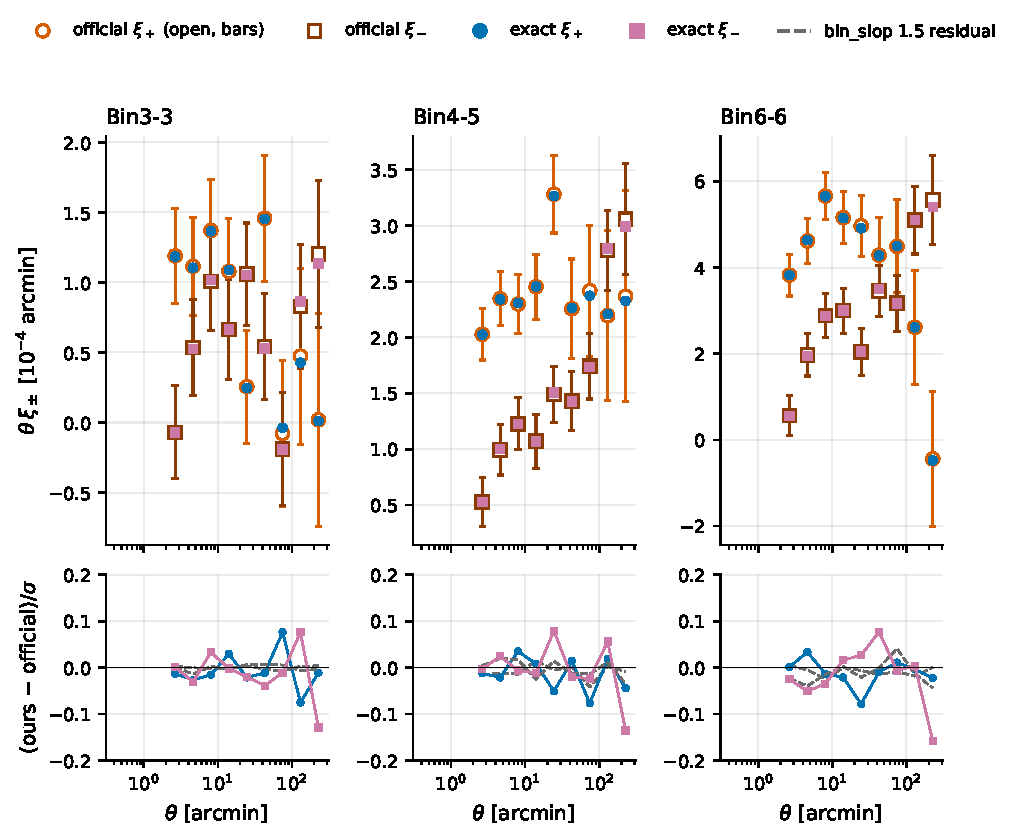
\includegraphics[width=\textwidth]{figs/fig_xipm.pdf}
\caption{$\theta\xi_\pm$ in the 9 official bins (top) and the difference from the release in units of $\sigma_{\rm official}$ (bottom). The \texttt{bin\_slop} 1.5 product (dashed) lies on the official points; the exact run (solid) moves by at most $0.17\sigma$. Not gated.}\label{fig:xi}
\end{figure}
\begin{figure}[!ht]\centering
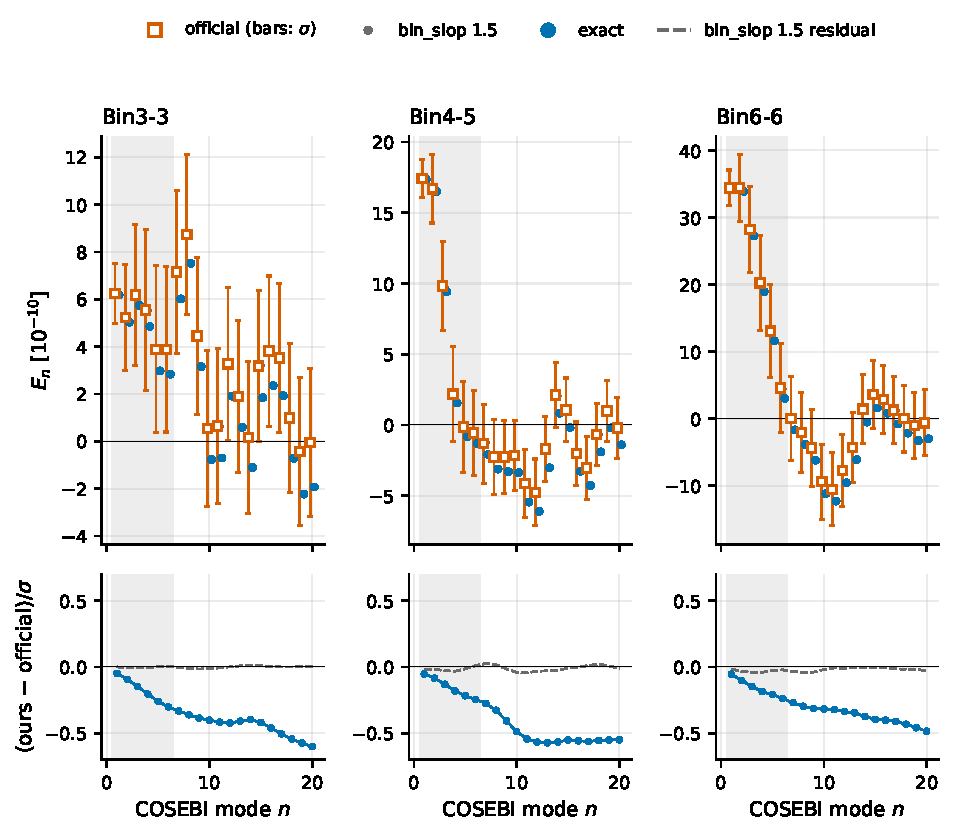
\includegraphics[width=\textwidth]{figs/fig_cosebis.pdf}
\caption{COSEBIs $E_n$, modes 1--20 (grey band: analysis range $n\le6$), and the difference from the release in $\sigma$. The exact run drifts smoothly with $n$ (up to $0.6\sigma$ at $n=20$ in 3-3 and 4-5), mostly from the outermost fine bins at $\theta\approx290$--$300'$ where the COSEBI filters weight $\xi$ strongly; for $n\le6$ all three agree within $0.31\sigma$.}\label{fig:cos}
\end{figure}
\begin{figure}[!ht]\centering
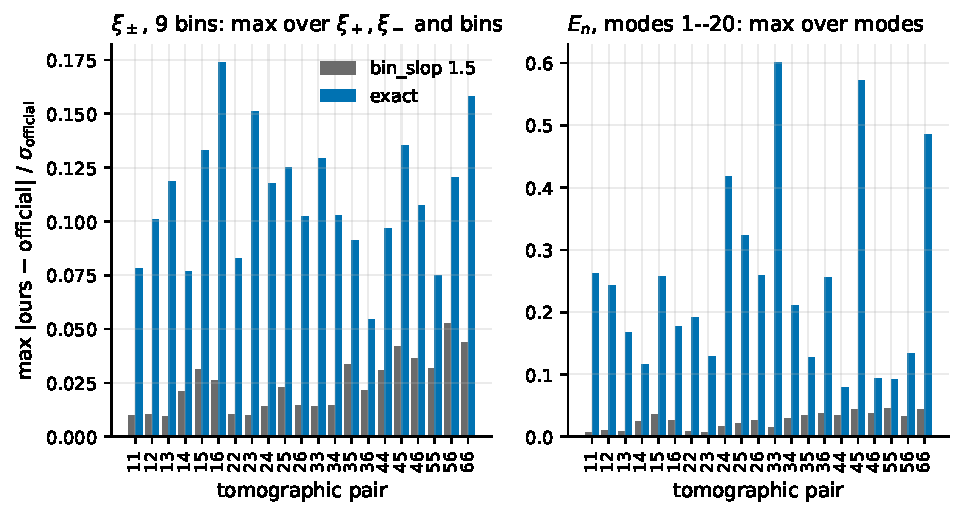
\includegraphics[width=\textwidth]{figs/fig_summary.pdf}
\caption{Maximum $|{\rm ours}-{\rm official}|/\sigma_{\rm official}$ for each of the 21 pairs. \texttt{bin\_slop} 1.5: $\xi_\pm$ 0.009--0.053, $E_n$ 0.007--0.046. Exact: $\xi_\pm$ 0.054--0.174, $E_n$ 0.080--0.601. The release used \texttt{bin\_slop} 1.5, so the exact run differs from it by the size of that approximation; the model $\chi^2$ of $E_n$ (modes 1--6) at the release best fit changes from 127.23 (official) to 127.52 (1.5) and 127.71 (exact).}\label{fig:sum}
\end{figure}

\section{Theory chain}
The physical decomposition is the same; the granularity differs. Ours fuses the NLA and GG+GI+IG+II assembly into the Limber kernel (15 instead of 55 integrals, \file{docs/KCAP\_OVERVIEW.md}); the $n(z)$ shift is a separate step before Limber, as in the official chain.

\begin{tabularx}{\textwidth}{@{}>{\bfseries}p{2.6cm}YY@{}}
\toprule
Stage & Difference & Measured effect \\
\midrule
Linear $P(k)$ & Same CAMB; $N_{\rm eff}$ 3.044 vs 3.046 and $k$-grid 194 vs 215 nodes unquantified. & None known. \\
Non-linear (KV450) & Own HMcode-2016 re-implementation vs.\ CAMB ``mead''. & Max $|\Delta\chi^2|=0.12$ near the data; $\Delta S_8=-10^{-4}$. \\
Non-linear (Legacy) & Official: neural emulator replacing CAMB+HMcode-2020. Ours: direct CAMB with feedback. & $\chi^2$ residual on 3509 official samples: mean $-0.26$, std 0.79, max 6.7. Our docs attribute it to emulator error; untested. \\
Limber & Official: quadrature with $\sim10^{-3}$ noise and spline ringing $O(5\times10^{-4})$. Ours: smooth in parameters. & Not separately quantified. \\
IA & KV450: single-amplitude NLA, identical. Legacy: mass-dependent NLA; our form is inferred from $\chi^2$ tests, not read from source. & Alternatives rejected by $\Delta\chi^2$ of 16--47. \\
$C(\ell)\to\xi$ & Ours has both the kcap-style and an exact-bin route. & kcap route matches the spec to $\Delta\chi^2\le0.08$; default route to $\le0.56$. \\
COSEBIs from $C(\ell)$ & Same method (Bessel $W_n$ integral); filter roots with 8 digits. & Orthonormality $2.8\times10^{-7}$ over 20 modes. \\
Our emulator & Emulates the linear transfer function only; halo model stays exact. & $\Delta\ln L\le1.1\times10^{-3}$ on 200 posterior samples. \\
\bottomrule
\end{tabularx}

\section{Likelihood, covariance and priors}
\begin{itemize}
\item \textbf{KV450 data and covariance} are byte-identical (same md5, same 195-point vector and cuts); our implementation hard-codes the index constants, theirs reads the ini.
\item \textbf{Likelihood form:} plain Gaussian $\chi^2$ in both. Ours solves via a Cholesky factor (checked against the explicit inverse to $\le10^{-10}$); the official MontePython likelihoods also use Cholesky, the CosmoSIS paths invert the matrix. The KV450 fiducial run applies no Hartlap factor (\file{mini\_2pt\_like.py}); other kcap modules offer one.
\item \textbf{Covariance construction} (Legacy: Reischke et al.\ 2025, described in the release README) is not implemented by us. We therefore cannot propagate our own DR5 measurement into a likelihood.
\item \textbf{Priors:} KV450 identical. Legacy samples $S_8$ with correlated photo-$z$ shifts and mass-dependent IA nuisance parameters; ours lacks this layer (the shift covariance is loaded but unused), so a Legacy posterior cannot yet be sampled with our stack.
\item \textbf{Legacy validation:} $\chi^2=127.23$ (official data) versus 127.29 (chain) at the best-posterior point, 126 $E_n$ points. Reweighting the official chain with our likelihood moves $S_8$ from 0.8128 to 0.8142.
\item \textbf{Blinding} is a data-product choice outside the likelihood in both pipelines.
\end{itemize}

\section{What exists on one side only}
\begin{tabularx}{\textwidth}{@{}YY@{}}
\toprule
Only in the official pipeline & Only in \texttt{kidspipe} \\
\midrule
Covariance construction; band powers; 3$\times$2pt and BOSS likelihoods; Legacy $S_8$ sampling and correlated priors; module-level configuration. & Emulator of the linear transfer function; stage caches and blocked fast/slow sampling; independent KD-tree pair counter (agrees with TreeCorr to 0.05$\sigma$, limited to 0.25\% of galaxies and $\theta\le60'$); chunked exact-measurement driver (all 21 pairs, 39.3\,h; can now be spread over MPI ranks); exact-vs-\texttt{bin\_slop} comparison tools. \\
\bottomrule
\end{tabularx}

\section{Conclusion}
For the COSEBIs and $\xi_\pm$ likelihoods we share, the architectural differences do not change the numbers beyond the quoted small effects. The practical limits are on our side: no covariance code, no configuration-level extensibility, and no Legacy prior layer. Items to settle if a closer comparison is needed: a TreeCorr 4.2.3 run on a subsample, the cause of the Legacy $\chi^2$ scatter (emulator versus other), and a measured (not estimated) kcap timing.

\vspace{4pt}\footnotesize\sloppy
Sources: \file{docs/KCAP\_OVERVIEW.md}, \file{docs/DESIGN.md}, \file{docs/USAGE.md} (MPI), \file{runs/dr5\_measure/RESUME.md} (item 9), CosmoSIS \file{runtime/mpi\_pool.py}, \file{docs/PERFORMANCE.md}, \file{docs/RESULTS.md}, \file{docs/KIDS\_LEGACY\_REVIEW.md}, \file{docs/DR5\_MEASUREMENT\_REPORT.md}, \file{reference/kcap}, release README and ini files.
\end{document}
